% F091｜完全立方数的立方根尾数速判｜06_summary.tex
% 继承上传模板的 LaTeX 环境；当前条目的内容独立编写。
\clearpage
\begin{summarybox}
\textbf{\textcolor{CSummary}{快记、快懂、快用}}
\par\medskip
\begin{center}
% F091｜split 原创简明教学示意图
\begin{tikzpicture}[>=stealth,scale=.9]
\node[draw,rounded corners,fill=teal!9,minimum width=2.5cm,minimum height=1.25cm] (a) at (0,0){$\underbrace{103}_{\text{高位}}\mid\underbrace{823}_{\text{低位}}$};
\node[draw,rounded corners,fill=orange!9,minimum width=3.2cm,minimum height=1.25cm] (b) at (4.5,0){$4^3\le103<5^3$};
\node[draw,rounded corners,fill=teal!15,minimum width=2.3cm,minimum height=1.25cm] (c) at (9.0,0){$\sqrt[3]{103823}=47$};
\draw[->,thick] (a)--(b);\draw[->,thick] (b)--(c);
\node at (4.5,-1.2){\small 高位定十位，末位定个位};
\end{tikzpicture}

\end{center}
\medskip
\textbf{快记：}三位一组；左边定十位；最后一位定个位。\par\textbf{快懂：}立方展开后，个位只和原数个位有关。\par\textbf{快用：}已知某数是两位整数的立方时，十几秒可给出整数根并验算。
\end{summarybox}
\clearpage
\begin{summarybox}
\textbf{\textcolor{CSummary}{和近似立方根的区别}}
\par\medskip
\begin{center}
% F091｜verify 原创简明教学示意图
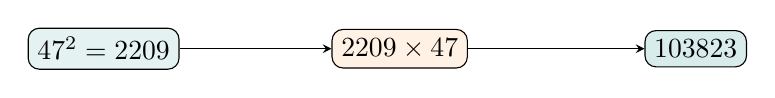
\begin{tikzpicture}[>=stealth,scale=.94]
\node[draw,fill=teal!10,rounded corners] (a) at (0,0){$47^2=2209$};
\node[draw,fill=orange!10,rounded corners] (b) at (4,0){$2209\times47$};
\node[draw,fill=teal!15,rounded corners] (c) at (8,0){$103823$};
\draw[->] (a)--(b);\draw[->] (b)--(c);
\end{tikzpicture}

\end{center}
\medskip
\textbf{完全立方：}本条用数位法找精确整数。\par\textbf{一般正数立方根：}F087 用切线迭代求近似小数；F092 给常用小立方数表。
\end{summarybox}
